\documentclass{beamer}
% This is presentation for InterMine community meeting talk
% Author: Asher Pasha
% Date: January 2020
% Usage (OpenBSD 6.6, Mate 1.22.1): pdflatex Asher_ThaleMine.tex; atril Asher_ThaleMine.pdf

% Make footnote tiny
\setbeamerfont{footnote}{size=\tiny}

\usepackage{graphicx}

% Package for URLs
\usepackage{hyperref}
\definecolor{beamerblue}{rgb}{0.2,0.2,0.7}
\hypersetup{colorlinks=true,urlcolor=beamerblue,citecolor=beamerblue}

% Citations
\usepackage[style=authoryear,backend=bibtex]{biblatex}
\bibliography{Asher_ThaleMine}

\begin{document}
\title[BAR ThaleMine] 
{BAR ThaleMine}
\author[Pasha, Provart]{Asher Pasha\inst{1} \and Nicholas Provart\inst{1}}
\institute[University of Toronto] 
{
    \inst{1}
    Bio-Analytic Resource (BAR)\\
    Centre for the Analysis of Genome Evolution and Function\\
    University of Toronto\\
    Toronto, Canada
}
\date{\today}

\frame{\titlepage}

\begin{frame}
    \frametitle{BAR: Bio-Analytic Resource}
    About us:
    \begin{itemize}
        \item One of the largest Plant Biology Resources
            %\item Paper published in 2005\footnote{\href{http://dx.doi.org/10.1111/j.1365-313X.2005.02437.x}{\tiny{Toufighi \emph{et al}., 2005}}}
            %\item Paper published in 2005\myref{http://dx.doi.org/10.1111/j.1365-313X.2005.02437.x}{Toufighi \emph{et al}., 2005}
        \item Paper published in 2005\footcite{bar2005}
        \item Based in University of Toronto, Canada
        \item Free to access: \href{http://bar.utoronto.ca}{http://bar.utoronto.ca}
    \end{itemize}
    Resources Include:
    \begin{itemize}
        \item Web applications, web services, databases
        \item Gene Expression data (\href{http://bar.utoronto.ca/efp}{eFP}, \href{http://bar.utoronto.ca/eplant}{ePlant})
        \item Protein-Protein, Protein-DNA Interactions (\href{http://bar.utoronto.ca/interactions2}{AIV2})
        \item Protein structures (ePlant)
    \end{itemize}
\end{frame}

\begin{frame}
    \frametitle{Araport: Arabidopsis Information Portal}
    A centralized resource for Arabidopsis data\footcite{araport2015}
    \begin{itemize}
        \item Started in 2013 under the leadership of Prof. Chris Town (JCVI)
        \item JCVI, TACC, University of Cambridge
        \item Drupal 7 based \href{http://araport.org}{araport.org} page
        \item ThaleMine (InterMine instance)
        \item App store on araport.org
        \item \href{https://apps.araport.org/jbrowse/?data=arabidopsis}{JBrowse}
        \item Araport11 re-annotation project
        \item Single Sign on to all Araport resources
        \item RESTful API for scientific data
        \item Community outreach (workshops, conferences, etc)
    \end{itemize}
\end{frame}

\begin{frame}
    \frametitle{Araport: Arabidopsis Information Portal}
    \begin{figure}[H]
        \centering
        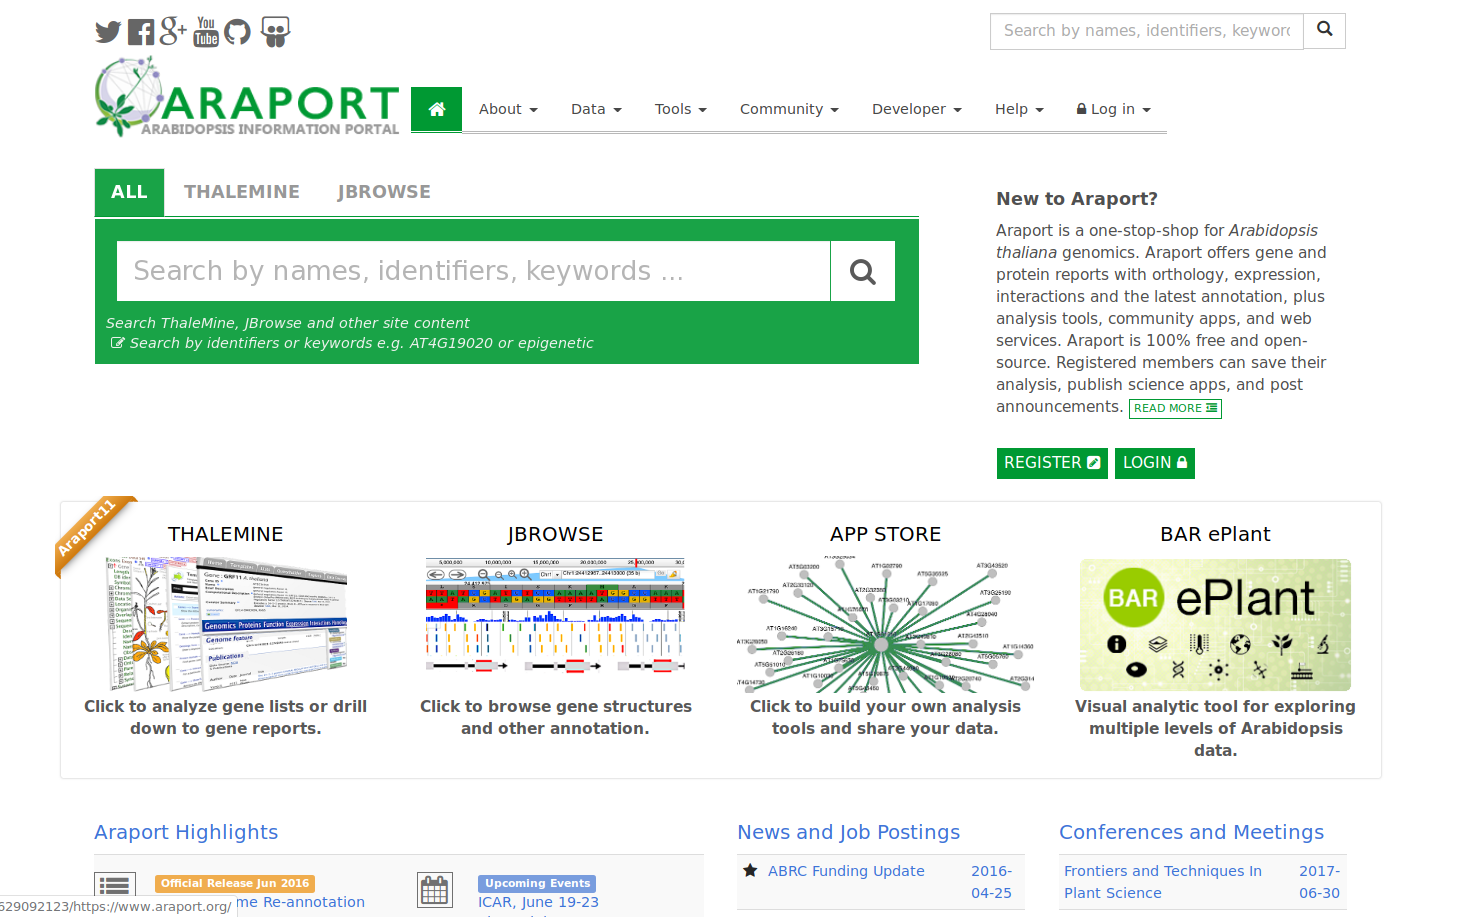
\includegraphics[width=\columnwidth]{img/Araport2017.png}
    \end{figure}
\end{frame}

\begin{frame}
    \frametitle{Araport: Arabidopsis Information Portal}
    BAR contibution to Araport
    \begin{itemize}
        \item Provided gene expression database used by BAR eFP Arabidopsis Browser
        \item Attended Araport workshop/hackathon in November 2014
        \item Interactions Viewer - the first community app published on Araport.org
        \item Contributed serveral apps and APIs over the next few years.
        \item Biggest contribution: BAR ePlant app.
    \end{itemize}
\end{frame}

\begin{frame}
    \frametitle{Araport: Arabidopsis Information Portal}
    Funding status
    \begin{itemize}
        \item Lost all funding in 2016
        \item Lost almost all staff 
        \item New application for funding failed
    \end{itemize}
    Future of Araport team
    \begin{itemize}
        \item JCVI, TACC, BAR, TAIR, NCGR
        \item First meeting at JCVI in March, 2019
        \item BAR got ThaleMine, TAIR got JBrowse, NCGR contributed GCV
        \item Every thing else was depricated
        \item News Update: araport.org
    \end{itemize}
\end{frame}

\begin{frame}
    \frametitle{Araport ThaleMine to BAR ThaleMine}
    Araport ThaleMine: A few minor problems
    \begin{itemize}
        \item Not maintained since 2017
        \item Based on InterMine 1.8.5
        \item Used modified data
        \item Used several custom loader and displayers
        \item Some InterMine core and biosource changes where never made upstreams
        \item To difficult to upgrade to InterMine 3.1.2
    \end{itemize}
\end{frame}

\begin{frame}
    \frametitle{BAR ThaleMine: Principles}
    No initial funding. So we follow these rules
    \begin{description}
        \item [Simplicity] Keep code to minimum possible lines and contribute as many changes to InterMine (upstream) as possible.
        \item [Least Surprise] Test and upgrade every minor release (Principle of least astonishment)
        \item [Clarity] No modification to data
        \item [Extensibility] Build for the future (Java 11, etc)
        \item [Parsimony] Write loaders and displayers only when we have to.
    \end{description}
\end{frame}

\begin{frame}
    \frametitle{BAR ThaleMine}
    \begin{itemize}
        \item We started from scratch (using make mine script)
        \item Based on Humanmine, FlyMine, and Araport ThaleMine
        \item Got most of the loaders working
        \item Pushed changed to upstream InterMine
        \item So far: ThaleMine v4.1.2-20200127
        \item Also on GitHub ThaleMine and ThaleMine Bio Sources
    \end{itemize}
\end{frame}

\begin{frame}
    \frametitle{BAR ThaleMine: What's working}
    \begin{itemize}
        \item data categories figure
        \item
    \end{itemize}
\end{frame}

\begin{frame}
    \frametitle{BAR ThaleMine: Some future plans and Known Issues}
    The follow is planned
    \begin{itemize}
        \item Arabidopsis Strains
        \item Gene expression data (Araport11 RNA-Seq)
        \item Salk data (TDNA-Seq)
        \item Gene histories
        \item TAIR annotations
    \end{itemize}
    Known Issues
    \begin{itemize}
        \item web properties from ThaleMine web service
        \item Bluegene frontend
    \end{itemize}
\end{frame}

\begin{frame}
    \frametitle{Acknowledgements}
\end{frame}

\end{document}
